
\clearpage
\section{Criteria for goodness-of-fit}
All criteria shown below for testing the goodness of a fit should be
considered with caution \cite{Bevington2003,Press2007}.
When you get data on a SAS instrument
the measured intensities are measured with some statistical uncertainties.
Normally one assumes Poisson statistics to determine the uncertainty
in the counting statistics. The data reduction software should than perform a
proper error propagation analysis for all succeeding data treatment operations.
However, by this procedure only statistical uncertainties are taken into account.
All systematic uncertainties are then hopefully covered during the data treatment,
as for example background correction, transmission correction etc \ref{ch:SASdatacorrection}.
~\\
\subsection{chi square test}
~\\
The method of least squares is built on the hypothesis that the
optimum description of a set of data is one which minimizes the
weighted sum of squares of deviations, between the data,
$I_\text{exp}(q_i)$ , and the fitting function $I_\text{th}(q_i)$:
\begin{equation}
\chi^2 = \displaystyle\sum_{i=1}^N
\left(\frac{I_\text{exp}(q_i)-I_\text{th}(q_i)}{\Delta
I(q_i)}\right)^2
\label{eq:chi2}
\end{equation}
As a rule of thumb for chi-square fitting is the statement that a
good fit is achieved when the reduced chi-square equals one. The
reduced chi-square value, which equals the residual sum of square
divided by the degree of freedom can be computed by
\begin{equation}
\chi^2_\nu = \displaystyle \frac{1}{N-m} \sum_{i=1}^N
\left(\frac{I_\text{exp}(q_i)-I_\text{th}(q_i)}{\Delta
I(q_i)}\right)^2 = \frac{\chi^2}{N-m}
\end{equation}
where $N$ is the number of data points and $m$ the number of fit parameters.
$\nu=N-m$ is called the "number of degree of freedom". The reduced chi-square
is closely related to the variance of the fit $s^2$ by
\begin{equation}
s^2=\chi_\nu^2 \left( \frac{1}{N}\sum_{i=1}^N \frac{1}{\left(\Delta I_i^\text{exp}\right)^2}\right)^{-1}
\end{equation}

In the theory of hypothesis testing $\chi^2$ can be used to test
for goodness of a fit. The probability that a random set of $N$ data points
would yield a value of $\chi^2$ equal or greater than the measured
one is given by
\begin{equation}
\displaystyle Q_\text{factor} =
Q\left(\frac{N-m}{2},\frac{\chi^2}{2}\right) =
\frac{\Gamma\left(\frac{N-m}{2},\frac{\chi^2}{2}\right)}{\Gamma\left(\frac{N-m}{2}\right)}
\text{ with } \Gamma\left(a,x\right) =  \int_x^\infty t^{a-1}e^{-t}
dt
\end{equation}
For a fitting function being a good approximation to the data the experimental
value of $\chi^2_\nu$ should be close to one and the probability
$Q_\text{factor}$ somewhere between 0.01 and 0.5. For probability values
close to one the fit seems to be too good to be true.

\vspace{5mm}

The interpretation of the parameter $Q_\text{factor}$ can be summarized as:

\vspace{5mm}

\uline{\bf goodness-of-fit parameter: $Q_\text{factor}$}
\begin{description}
 \item[$Q_\text{factor}>0.99$] too good
 \item[$Q_\text{factor}>0.1$] believable
 \item[$Q_\text{factor}>0.001$] may be acceptable
 \item[$Q_\text{factor}<0.001$] questionable
\end{description}

\vspace{5mm}

The $Q_\text{factor}$-parameter is calculated after each calculation of the scattering curve together with $\chi^2_\nu$ and $s^2$. They are displayed and updated in the red marked area of the screen shot shown in fig.\ \ref{fig:GoodnessParGUI}.

~\\
\subsection{R-factor}
~\\
The crystallographers have introduced another parameter for the goodness of a fit.
They use the $R$ factor \cite{Rfactor,Hamilton1965} as a measure of model quality which is defined as
\begin{equation}\label{eqRfactor}
  R  \displaystyle  = \frac{\displaystyle\sum_{i=1}^N
\abs{\abs{I_\text{exp}(q_i)} -
\abs{I_\text{th}(q_i)}}}{\displaystyle\sum_{i=1}^N
\abs{I_\text{exp}(q_i)}}
\end{equation}
Theoretical values of $R$ range from zero (perfect
agreement of calculated and observed intensities) to infinity.  $R$
factors greater than 0.5 indicate in crystallography very poor
agreement between observed and calculated intensities. Models
refining to $R < 0.05$ are often considered to be good. However, the
$R$ factor must always be treated with caution, only as an indicator of
precision and not accuracy. In Crystallography partially incorrect
structures have been reported with $R$ values below $0.1$; many
imprecise but essentially correct structures have been reported with
higher $R$ values.

In practice, weighted $R$ factors $R_\text{w}$ are more often used
to track least-squares refinement, since the functions minimized are
weighted according to estimates of the precision of the measured
quantity. The weighted residuals are defined as:
\begin{equation} \displaystyle R_{w} =
\sqrt{\frac{\displaystyle\sum_{i=1}^N \left(\frac{\abs{I_\text{exp}(q_i)}
- \abs{I_\text{th}(q_i)}}{\Delta
I(q_i)}\right)^2}{\displaystyle\sum_{i=1}^N
\frac{I_\text{exp}^2(q_i)}{\Delta I^2(q_i)}}}
\end{equation}


The interpretation of the parameters $R$ and $R_w$ can be summarized as:

\vspace{5mm}

\uline{\bf goodness-of-fit parameters: $R,R_w$}
\begin{description}
\item[$R,R_w>0.3$] questionable
\item[$0.1 > R,R_w >0.3$] may be acceptable
\item[$R,R_w<0.1$] believable
\end{description}

\vspace{5mm}

The parameters $R$ and $R_w$ are calculated like the $Q_\text{factor}$-parameter after each calculation of the scattering curve. They are displayed and updated together with other goodness-of-fit parameters in the red marked area of the screen shot shown in fig.\ \ref{fig:GoodnessParGUI}. The goodness-of-fit parameters are not minimized. The parameter which is minimized is the $\chi^2$-value, defined in eq.\ \ref{eq:chi2}. The other goodness-of-fit parameters are than calculated after each fitting step or after evaluating the theoretical scattering curve via the "Apply"-button.

\subsection{other methods to compare similarity or distance between theory and data}

\begin{itemize}
  \item  \href{https://en.wikipedia.org/wiki/Kullback%E2%80%93Leibler_divergence}{Kullback-Leibler divergency} and  \href{https://en.wikipedia.org/wiki/Jensen%E2%80%93Shannon_divergence}{Jensen–Shannon divergence}
\begin{align}
    D_\mathrm{KL}(P\|Q)&=\sum_{i=1}^np_i\log {\frac{p_i}{q_i}}-p_i+q_i \\
    D_\mathrm{JS}(P\|Q)&=\frac12 D_\mathrm{KL}(P\|Q)+\frac12 D_\mathrm{KL}(Q\|P) \nonumber \\
                       &=\frac12 \sum_{i=1}^n \left(p_i-q_i\right)\left(\log p_i - \log q_i\right)
\end{align}
  \item  \href{https://en.wikipedia.org/wiki/Chi-squared_divergence}{chi-squared divergence}
\begin{align}
    D_{\chi^2}&= \sum_{i=1}^n\frac{\left(p_i-q_i\right)^2}{q_i}
\end{align}
  \item \href{https://en.wikipedia.org/wiki/Hellinger_distance}{Hellinger distance}
\begin{align}
    H(P,Q)&={\frac {1}{\sqrt {2}}}\;{\sqrt {\sum _{i=1}^{k}({\sqrt {p_{i}}}-{\sqrt {q_{i}}})^{2}}}
\end{align}
  \item \href{https://en.wikipedia.org/wiki/Hellinger_distance}{squared Hellinger distance}
\begin{align}
    H^{2}(P,Q)&=1-\sum_{i=1}^{k}{\sqrt {p_{i}q_{i}}}
\end{align}
  \item  \href{https://en.wikipedia.org/wiki/R%C3%A9nyi_entropy#R%C3%A9nyi_divergence}{Rényi divergence of order $\alpha$}:
\begin{align}
    D_{\alpha }(P\|Q)&={\frac {1}{\alpha -1}}\log \left(\sum _{i=1}^{n}{\frac {p_{i}^{\alpha }}{q_{i}^{\alpha -1}}}\right)
\end{align}
    \begin{description}
        \item[$\alpha=0$] $D_{0}(P\|Q)=-\log Q(\{i:p_{i}>0\})$ : minus the log probability under $Q$ that $p_i > 0$
        \item[$\alpha=1/2$] $D_{1/2}(P\|Q)=-2\log \sum_{i=1}^n\sqrt{p_iq_i}$ : minus twice the logarithm of the Bhattacharyya coefficient; (Nielsen \& Boltz (2010))
        \item[$\alpha=1$] $D_{1}(P\|Q)=\sum_{i=1}^np_i\log {\frac{p_i}{q_i}}$ : the Kullback–Leibler divergence;
        \item[$\alpha=2$] $D_{2}(P\|Q)=\log {\Big \langle }{\frac {p_{i}}{q_{i}}}{\Big \rangle }$ : the log of the expected ratio of the probabilities
        \item[$\alpha=\infty$] $D_\infty (P\|Q)=\log \sup_i\frac {p_i}{q_i}$ : the log of the maximum ratio of the probabilities
    \end{description}
  \item \href{https://github.com/stegua/ot1d}{Wasserstein distance} %https://pkomiske.github.io/Wasserstein/ %https://visualstudiomagazine.com/articles/2021/08/16/wasserstein-distance.aspx
  \item \href{https://en.wikipedia.org/wiki/Canberra_distance}{Canberra distance}:
\begin{align}
    D_{CD}&= \sum_{i=1}^n\frac{\abs{p_i-q_i}}{\abs{p_i}+\abs{q_i}}
\end{align}
  \item \href{https://en.wikipedia.org/wiki/Cosine_similarity}{Cosine distance}
\begin{align}
    D_{\cos}&= 1-\frac{\sum_{i=1}^n p_iq_i}{\sqrt{\sum_{i=1}^n p_i^2}\sqrt{\sum_{i=1}^n q_i^2}}
\end{align}

\end{itemize}


\begin{figure}[htb]
\begin{center}
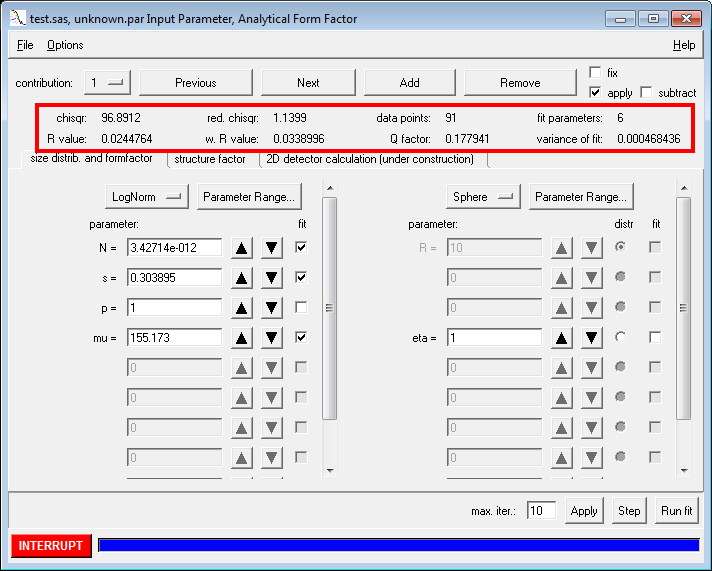
\includegraphics[width=0.712\textwidth]{../images/related_pages/goodnessOFfitPAR.png}
\end{center}
\caption{The parameters $Q, R,R_w$, describing the goodness of the fit, are displayed in the marked area of the GUI}
\label{fig:GoodnessParGUI}
\end{figure}

%~\\
\subsection{Confidence interval of the fitting parameter}
~\\

The confidence intervals of the fitting parameters are calculated at the minimum of the $\chi^2$. At the minimum first the partial derivatives according to the fit parameters $a_i$ are calculated to get the matrix elements $A_{kl}$ via
\begin{align}
A_{kl} &= \sum_{i=1}^{N} \frac{1}{\left(\Delta I_i^\mathrm{th}\right)^2} \frac{\partial I_i^\mathrm{th}(q_i,\mathbf{a})}{\partial a_k} \frac{\partial I_i^\mathrm{th}(q_i,\mathbf{a})}{\partial a_l}
\end{align}
The inversion of this matrix yield the covariance matrix
\begin{align}
        \mathbf{C} &= \mathbf{A}^{-1}
\end{align}
The standard deviations $\Delta a_i$ of the best-fit parameters are given by the square root of the corresponding diagonal elements of the covariance matrix
\begin{align}
\Delta a_i &= \sqrt{C_{ii}}
\end{align}
The correlation coefficient of the fit parameters $a_k$ and $a_l$ are given by
\begin{align}
r_{kl} &= \frac{C_{kl}}{\sqrt{C_{kk}C_{ll}}} = \frac{C_{kl}}{\Delta a_k \Delta a_l}
\end{align}
Both the non-diagonal elements of the correlation matrix $r_{k>l}$ and the confidence intervals of the fitting parameters $\Delta a_k$ are calculated when the fit converges and displayed in a GUI (fig.\ \ref{fig:ErrorGUI}) which can be opened via a menu button as shown in fig.\ \ref{fig:ErrorButton}.

\begin{figure}[htb]
\captionsetup[subfigure]{position=b}
\centering
\subcaptionbox{menu button showing the GUI for the confidence intervals and correlation matrix \label{fig:ErrorButton} }{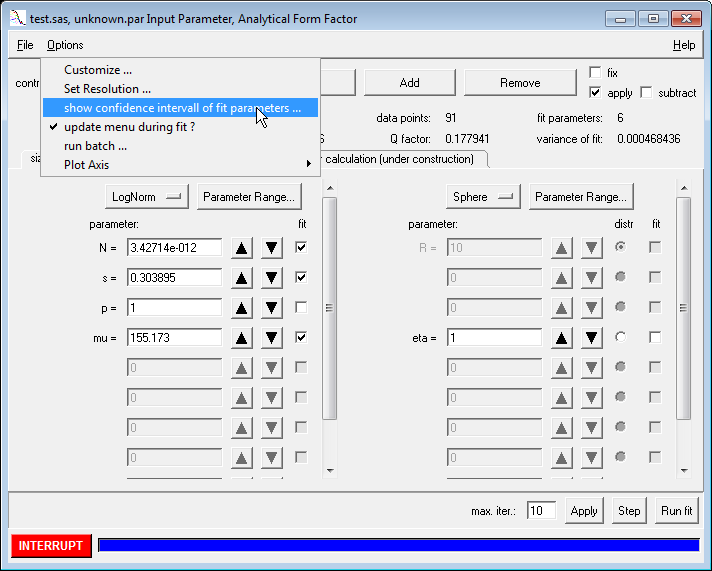
\includegraphics[width=0.47\textwidth]{../images/related_pages/menueConfidenceIntervall.png}}
\hfill
\subcaptionbox{GUI displaying the fitting parameters including confidence intervals and correlation matrix \label{fig:ErrorGUI} }{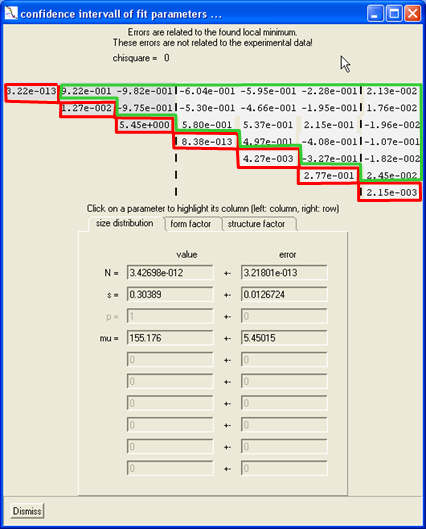
\includegraphics[width=0.47\textwidth]{../images/related_pages/ConfidenceIntervallANDCorrelationMatrix.png}}
\caption{The confidence intervals are calculated at the end of the minimization procedure.}
\label{fig:FitErrors}
\end{figure}

The routine can give nonphysical confidence intervals if
\begin{itemize}
\item no proper error bar for the experimental data are supplied
\item a wrong physical model for describing the data is used
\item the physical model has strongly correlated parameters
\begin{subequations}
\begin{align}
r_{kl} &\approx 0, a_k \mbox{ and } a_l \mbox{ are uncorrelated parameters} \\
r_{kl} &\approx \pm 1, a_k \mbox{ and } a_l \mbox{ are strongly correlated parameters}
\end{align}
\end{subequations}
\end{itemize}

The given value for the confidence interval of the fit parameters should not be used in the cases
\begin{itemize}
\item where the error is not normal distributed
\item where the data is given without error bar
\item where parameters are strongly correlated
\end{itemize}

\clearpage
\section{references to numerical strategies \SASfit make use of}
In small angle scattering analysis numerical integrations tools are used regularly. To get the scattering amplitude a 3D Fourier transform needs to be calculated, which simplifies to lower dimensional integrals in case of point symmetric, spherical symmetric, cylindrical symmetric or planar objects. For non-spherical symmetric shapes typically an average over the orientation distribution needs to be performed. Furthermore for systems with a size distribution an additional smearing over those distributions are essential. For SESANS data a Hankel transformation is required. In case of multiple scattering both a forward and as well as inverse Hankel transform are necessary. It has turned out, that each of these tasks might require a specialized integration routine to be efficient. Efficiency or parallelization becomes in the end essential if several of these integrations have to be solved numerically.

\subsection{Integrals for Form Factors} ~\\

To calculate the general case of a form factor of an object a 3D Fourier transform needs to be performed. When $\eta(\mathbf{r})$ is the scattering length density distribution of the scatterer the scattering amplitude $F(\mathbf{Q})$ is
\begin{align}
F(\mathbf{Q}) &= \int\!\! \int\!\! \int \eta(\mathbf{r}) e^{\imath \mathbf{Q}\mathbf{r}}\,\mathrm{d}\mathbf{r}
\end{align}
For objects with a point symmetric shape the integral simplifies to $\cos$ transform, which is real valued and not anymore complex and for which specialized algorithms are available \cite{Burkardt,Ooura1996,Chase1969,Ooura_1991,Team2024,Team2024a}
\begin{align}
F(\mathbf{Q}) &= \int\!\! \int\!\! \int \eta(\mathbf{r}) \cos\left( \mathbf{Q}\mathbf{r} \right)\,\mathrm{d}\mathbf{r}
\end{align}
For higher symmetric shapes the 3D Fourier transform simplifies further to lower dimensional integrals.

For spherical symmetric shapes one just needs to calculate
\begin{align}
F(Q) &= \int_0^\infty 4\pi r^2 \eta(r) \frac{\sin \left(Qr \right)}{Qr} \, \mathrm{d}r
\end{align}
which now only depend on the modulus of $Q$ and $r$. In this case a $\sin$ transform needs to be calculated. In all cases the integral has to be performed over an oscillating $\cos$ or $\sin$ function, which in the above two cases also have a constant oscillation frequency. Efficient algorithms can be found e.g. at \cite{Burkardt,Ooura1996,Chase1969,Ooura_1991,Team2024,Team2024a}

For cylindrical and point symmetric objects the Fourier transform reads as
\begin{align}
F(\mathbf{Q}) &= 2\pi\int_{-\infty}^{\infty}\cos(Q_zz) \int_0^\infty
\Delta\eta_\textrm{cyl}(r,z) \textrm{J}_0(Q_rr)r \,
\textrm{d}r \textrm{d}z
\end{align}
The integration over $z$ is still a $\cos$ transform, whereas the integration over the other two direction turn into a Hankel transform. The Bessel function also oscillates around zero but not with a fixed frequency. The roots are not analytically known which means some additional efforts for numerically evaluating them. The form factor of a homogeneous cylinder of length $L$ and radius $R$ oriented with the cylinder axis in $z$-direction therefore reads as
\begin{subequations}
\begin{align}
F_\mathrm{cyl}(\mathbf{Q}) &= 2\pi\int_{-L/2}^{L/2}\cos(Q_zz) \int_0^R
 \textrm{J}_0(Q_rr)r \,
\textrm{d}r \textrm{d}z \label{eq:FcosHankel}\\
&= \frac{\sin(Q_zL/2)}{Q_zL/2} \pi R^2L\frac{2\textrm{J}_1(Q_rR)}{Q_rR}  \label{eq:FcylOriented}
\end{align}
with
\begin{align}
\mathbf{Q} &= \begin{pmatrix}
                 Q_r \cos(\phi) \\
                 Q_r \sin(\phi) \\
                 Q_z \\
               \end{pmatrix}
\end{align}
\end{subequations}
In case of a homogeneous cylinder the $\cos$ and Hankel transform can be calculated analytically. For other more realistic models the integrations needs to be performed numerically. Algorithms for the $\cos$ transform already have been mentioned. For the Hankel transform several strategies have been discussed and used \cite{Chave1983,Anderson1989,Ooura_1991,Guptasarma1997,Ogata2005,Kong2007,Key2012,Kang2021}
From these algorithms especially the one from \cite{Ooura_1991} and \cite{Chave1983} are those which  both are fast as well as able to perform the transform with a given precision. The integral in eq.\ \ref{eq:FcosHankel} likely would gain using different quadrature strategies for $\int\mathrm{d}r$ (optimized Hankel transform quadrature \cite{Chave1983}) and $\int\mathrm{d}z$ (e.g.\ double exponential quadrature \cite{Mori2001,Mori1990}), i.e.\ a quadrature rule from a product of distinct optimum 1D quadrature rules needs to be investigated.

\subsection{Orientational and Size Distribution} ~\\

To calculate scattering pattern of particles with orientational (o) and size distribution (s) the scattering intensity $I=\langle \vert F\vert^2\rangle_\mathrm{o,s}$ has to averaged in case of non interacting particles. $\langle \rangle_\mathrm{o,s}$ denotes a multiple quadrature over the orientation and size probability function. In case of interacting particles both the averages of scattering intensities $I=\langle \vert F\vert^2\rangle_\mathrm{o,s}$ of a single particle  as well as the averages of the scattering amplitude $\vert\langle F\rangle_\mathrm{o,s}\vert^2$ of them are typically required.

In case of an averaged amplitude $\langle F\rangle_\mathrm{o,s}$ the integrals over a 3D hyper cube can be extended to the required $n$-dimensional hypercube including orientational as well size distribution. The orientational distribution increases the dimension of the hyper cube by maximal 3 dimensions namely the three Euler angles. Distributions of the size can in principle have any number of dimensions depending on the parametrization. A three dimensional rectangular cuboidal multi shell can have many size parameters in its form factor, each having a distribution.

In contrast to the calculation of the average amplitude the calculating of the averaged intensity first needs a $\vert F(\mathbf{Q})\vert^2$ operation which avoids extending directly the strategies  for quadrature algorithms over a hyper cube to higher dimensions.
Size distribution and orientation distributions over $m$ parameters $a_i$ (with $\mathbf{a}=(a_1, \ldots, a_m)^T$) and over the Euler angles  $(\alpha,\beta,\gamma)$ with a common distribution $p(\mathbf{a},\alpha,\beta,\gamma)$ of the form factor are simply calculated by
\begin{multline} \label{eq:Fredholm}
 \frac{d\sigma(\mathbf{Q})}{d\Omega} = I(Q) = \left\langle \vert F(\mathbf{Q},\mathbf{a},\alpha,\beta,\gamma)\vert^2\right\rangle_{\mathrm{o},\mathrm{s}} = \\
 \idotsint  p(\mathbf{a},\alpha,\beta,\gamma) \vert F(\mathbf{Q},\mathbf{a},\alpha,\beta,\gamma)\vert^2 \, \mathrm{d}\mathbf{a} \, \mathrm{d}\alpha \, \mathrm{d}\beta \, \mathrm{d}\gamma
\end{multline}
The determination of the distribution function $p(\mathbf{a},\alpha,\beta,\gamma)$ is one of the core tasks in small angle scattering analysis. The integral in eq.\ \ref{eq:Fredholm} is a multidimensional Fredholm integral. The SASview as well SASfit packages try to solve this (ill-posed) integral equation by assuming analytical parametrized distribution functions to obtain the orientation and size distribution information. In many typical cases discussed in literature a size and  orientation distributions are assumed to be factorizable as
\begin{align}
p(\mathbf{a},\alpha,\beta,\gamma) &= p_\mathrm{o}(\alpha,\beta,\gamma)\prod_{i=1}^m p_{\mathrm{s},i}(a_i)
\end{align}
where the size distribution $p_{\mathrm{s},i}(a_i)$ is described in first approximation by a simple distribution function like a normal, lognorm, gamma, ... distribution and $p_\mathrm{o}(\alpha,\beta,\gamma)$ is describing the orientation distribution function in terms of Euler angles.


For cylindrical symmetric objects due to symmetry one integration around the symmetry axis can be done analytically, whereas the other two over the polar angles still might need to be performed numerically.
For integration over polar angles, i.e. over the surface of a unit sphere special algorithms are available like Lebedev quadrature \cite{Lebedev1975,Lebedev1976,Lebedev1977,Lebedev2003}, spherical designs \cite{Graef2011,Hardin1996}, or spherical Fibonacci point sets \cite{Marques_2013,Swinbank2006}. However, these methods have the disadvantage of having no error estimate of the integral, but on the other side they might be easily adapted for parallelization due to the known grid points.

A special case of orientation distribution is the fully random orientation distribution. For this case all direction between the scattering object and the vector $\mathbf{Q}$ are equal probable and an average over all direction of $\mathbf{Q}$ is equivalent to averaging over all 3 Euler angles. This means, that a random orientational average requires again an integration over a unit sphere. A symmetry constrain like a cylindrical symmetry of the particles would reduce the orientation average to a single integral. In case of a random oriented cylinder like in eq.\ \ref{eq:FcylOriented} the average reads as
\begin{multline}\label{eq.Fcyl_rndODF}
\vert\left\langle F_\mathrm{cyl}(\mathbf{Q})\vert^2\right\rangle_{\mathrm{rnd-o}} = \\
\int_0^{\pi/2} \left\vert \pi R^2L \frac{\sin(QL/2\cos(\theta))}{QL/2\cos(\theta)} \frac{2\textrm{J}_1(QR\sin(\theta))}{QR\sin(\theta)}\right\vert^2 \sin(\theta) \, \mathrm{d}\theta  \end{multline}
The kernel of this integral is an oscillating function, but it does not oscillate around zero as the kernel is strictly positive. Therefore certain integration strategies for oscillating functions can not be applied directly. We also have two oscillations, one depending on the length $QL/2$ and the other on $QR$. If the cylinder has additional size distributions in $L$ and $R$ the final multidimensional integral to be solved is
\begin{multline}\label{eq.Fcyl_rndODF}
\frac{d\sigma_{\mathrm{cyl},\mathrm{rnd-o},\mathrm{s}}(Q)}{d\Omega}=\left\langle \vert F_\mathrm{cyl}(\mathbf{Q})\vert^2\right\rangle_{\mathrm{rnd-o},\mathrm{s}} = \int_0^\infty \!\int_0^\infty \!\int_0^{\pi/2} p_\mathrm{s}(L,R) \quad \times\\
 \left\vert \pi R^2L \frac{\sin(QL/2\cos(\theta))}{QL/2\cos(\theta)} \frac{2\textrm{J}_1(QR\sin(\theta))}{QR\sin(\theta)}\right\vert^2 \sin(\theta) \, \mathrm{d}\theta  \, \mathrm{d}R\, \mathrm{d}L
\end{multline}
The integral kernel behaves well enough so that the order of the integrals can be changed. If the orientational average is done first, the resulting function in this case for $2R\approx L$ does not has anymore many oscillations and the outer integrations over $L$ and $R$ might be done easily with standard strategies for quadratures over hypercubes. However, for extreme aspect ratios this is not anymore valid.

\subsection{SESANS - MSAS - resolution function} ~\\
\subsubsection{SESANS} ~\\
In case of an isotropic scatterer the SESANS signal $\tilde{G}(\delta)$ is directly related to the SANS differential cross-section $\frac{d\sigma(Q)}{d\Omega}$ via a zero order Hankel transform \cite{Krouglov2003,Andersson2008,Kohlbrecher2017}which reads as
\begin{align}
\tilde{G}(\delta) &= \frac{1}{2\pi}\mathcal{H}_0\left[\frac{\mathrm{d}\sigma(Q)}{\mathrm{d}\Omega}\right](\delta)
= \frac{1}{2\pi} \int_{0}^{\infty} Q J_0(Q\delta) \frac{\mathrm{d}\sigma(Q)}{\mathrm{d}\Omega} \, \mathrm{d}Q
\end{align}
Coming back to the example of random oriented cylinders with size distributions for the length and radius we finally end up with
\begin{multline}  \label{eq.Fcyl_rndODF_SESANS}
\tilde{G}_{\mathrm{cyl},\mathrm{rnd-o},\mathrm{s}}(\delta) = \frac{1}{2\pi} \int_{0}^{q_\mathrm{max}} \! \int_0^\infty \!\int_0^\infty \!\int_0^{\pi/2} Q J_0(Q\delta) \, p_\mathrm{s}(L,R) \quad \times\\
 \left\vert \pi R^2L \frac{\sin(QL/2\cos(\theta))}{QL/2\cos(\theta)} \frac{2\textrm{J}_1(QR\sin(\theta))}{QR\sin(\theta)}\right\vert^2 \sin(\theta) \, \mathrm{d}\theta  \, \mathrm{d}R\, \mathrm{d}L \, \mathrm{d}Q
\end{multline}
As experimentally SESANS signals are only measured with a detector probing the polarization to a maximum value of $q_\mathrm{max}$, the Hankel transform might be significantly truncated. If in this case $\int_{0}^{q_\mathrm{max}} \mathrm{d}Q$ can be replaced by $\int_{0}^{\infty} \mathrm{d}Q-\int_{q_\mathrm{max}}^\infty \mathrm{d}Q$ or if a another routine preferable directly evaluates the integral  $\int_{0}^{q_\mathrm{max}} \mathrm{d}Q$ might depend on how many roots of the Bessel function are within the domain $[0,q_\mathrm{max}]$.

\subsubsection{Multiple Small Angle Scattering (MSAS)} ~\\

According to \cite{Schelten1980,Jensen2018} multiple  small angle scattering can be computed from the single scattering approximation via the intermediate function $i_1(r)$.
\begin{align}\label{eq:MSAS_SchmatzSchelten}
 i_1(r) &= 2\pi t \int_0^\infty J_0(qr) \frac{\mathrm{d}\sigma_1}{\mathrm{d}\Omega}(q) q \mathrm{d}q \\
 &=2\pi t \mathcal{H}_0\left[\frac{\mathrm{d}\sigma_1}{\mathrm{d}\Omega}(q)\right](r)= 4\pi^2 t \tilde{G}(r)\\
 i_m(r) &= e^{-i_1(0)/k_0^2}k_0^2\left(\exp\left(i_1(r)/k_0^2\right)-1\right) \\
        &= k_0^2\left[\exp\left(\frac{t}{k_0^2}\left(\tilde{G}(r)-\tilde{G}(0)\right)\right)-\exp\left(-\frac{t}{k_0^2}\tilde{G}(0)\right)\right] \label{eq:MSASim}\\
 \frac{\mathrm{d}\sigma_m}{\mathrm{d}\Omega}(q)&= \frac{1}{2\pi t} \int_0^\infty J_0(qr) i_m(r) r \mathrm{d}r = \frac{1}{2\pi t} \mathcal{H}_0\left[i_m(r)\right](q) \label{eq:MSAS}\\
 k_0 &= \frac{2\pi}{\lambda}
\end{align}
where $\frac{\mathrm{d}\sigma_m}{\mathrm{d}\Omega}(q)$ is the measured scattering cross-section including multiple scattering contributions normalized on the sample volume and  corrected for absorption and incoherent scattering, i.e. corrected for all beam attenuation effects except coherent small angle scattering. $\frac{\mathrm{d}\sigma_1}{\mathrm{d}\Omega}(q)$ is the corresponding single scattering cross-section per volume.
It can be seen, that the intermediate function $i_1(r)$ is except a pre-factor identical to the projected correlation function $\tilde{G}(r)$ used in the theory of  SESANS analysis,
$i_1(r)=\tilde{G}(r)\left(2\pi\right)^2t$.

What does this mean for the case of random oriented cylinders with a size distribution for the length and radius? Here we consider a system which would scatter that strong, that multiple scattering has to be considered. In this case first the correlation function in eq.\ \ref{eq.Fcyl_rndODF_SESANS} and afterwards the intermediate function including multiple scattering $i_m(r)$ is calculated. This functions then needs to be Hankel transformed again according to eq.\ \ref{eq:MSAS}. In total 5 nested numerical integration are required for the example of polydisperse random oriented cylinders.

%In the \texttt{SASfit} C-source code a function \texttt{sasfit\_hankel()} is supplied to perform a
%Hankel transform. It can be configured to use several different algorithms:
%\cite{Chave1983,Anderson1989,Ooura_1991,Guptasarma1997,Ogata2005,Kong2007,Key2012,Kang2021}
%From these algorithms especially the one from \cite{Ooura_1991} and \cite{Chave1983} are those which
%are both fast as well as able to perform the transform with a given precision.

%It would be interesting to compare those algorithm against newer ones, e.g.
%\cite{Liu2024,Xu2019,Diehl2024,Diehl2024a} for converting SANS cross sections into a SESANS intensity.

\subsubsection{Resolution Function} ~\\
If the resolution function needs to be included in the analysis eq.\ \ref{eq:MSAS} or eq.\ \ref{eq.Fcyl_rndODF} would need to be convoluted by a resolution function which would add another integral to the formula.

\subsection{Summary} ~\\

Already for a simple model of a polydisperse random oriented cylinder several nested integrals needs to be solved numerically.
A part of the integrals, like over a combined orientation and size distribution are calculated over a hyper cube. Adaptive algorithms have been discussed and supplied in \cite{Johnson2017,Genz1980,Berntsen1991,Bull1995}. However, in the present case integrals in certain dimensions might profit if they would be treated with different strategies, like Hankel transforms, integrals over oscillating but positive functions, or orientational averages over a unit sphere. The question would be, if quadrature rules with mixed strategies for the different dimensions can be developed. Ideally they should also be vectorizable for optional parallelization. For the given example of polydisperse random oriented cylinder performance test at the beginning using optimized one dimensional quadrature rules like for the Hankel transform or over strictly positive but oscillating functions might be useful, as those could immediately improve existing codes in SASview and SASfit.

To access in \SASfit the specialized integration routines the functions \texttt{sasfit\_integrate()}, \texttt{sasfit\_cubature()},
\texttt{sasfit\_orient\_avg()}, and \texttt{sasfit\_hankel()} are supplied.
\texttt{sasfit\_integrate()} performs one-dimensional integrations and \texttt{sasfit\_cubature()} multidimensional integrations over multi-dimensional cubes. \texttt{sasfit\_orient\_avg()} performs efficient integrations over the surface of a sphere to perform orientational averages. \texttt{sasfit\_hankel()} supplies highly optimized routines for Bessel or Hankel transforms containing oscillatory Bessel functions in the integrand. The window for fitting or simulating data (fig.\ \ref{fig:CustomizeIntGUI}) has a menu option under \texttt{[Options|Customize...]} opening a window to configure the internal integration routines.
\begin{figure}[htb]
\begin{center}
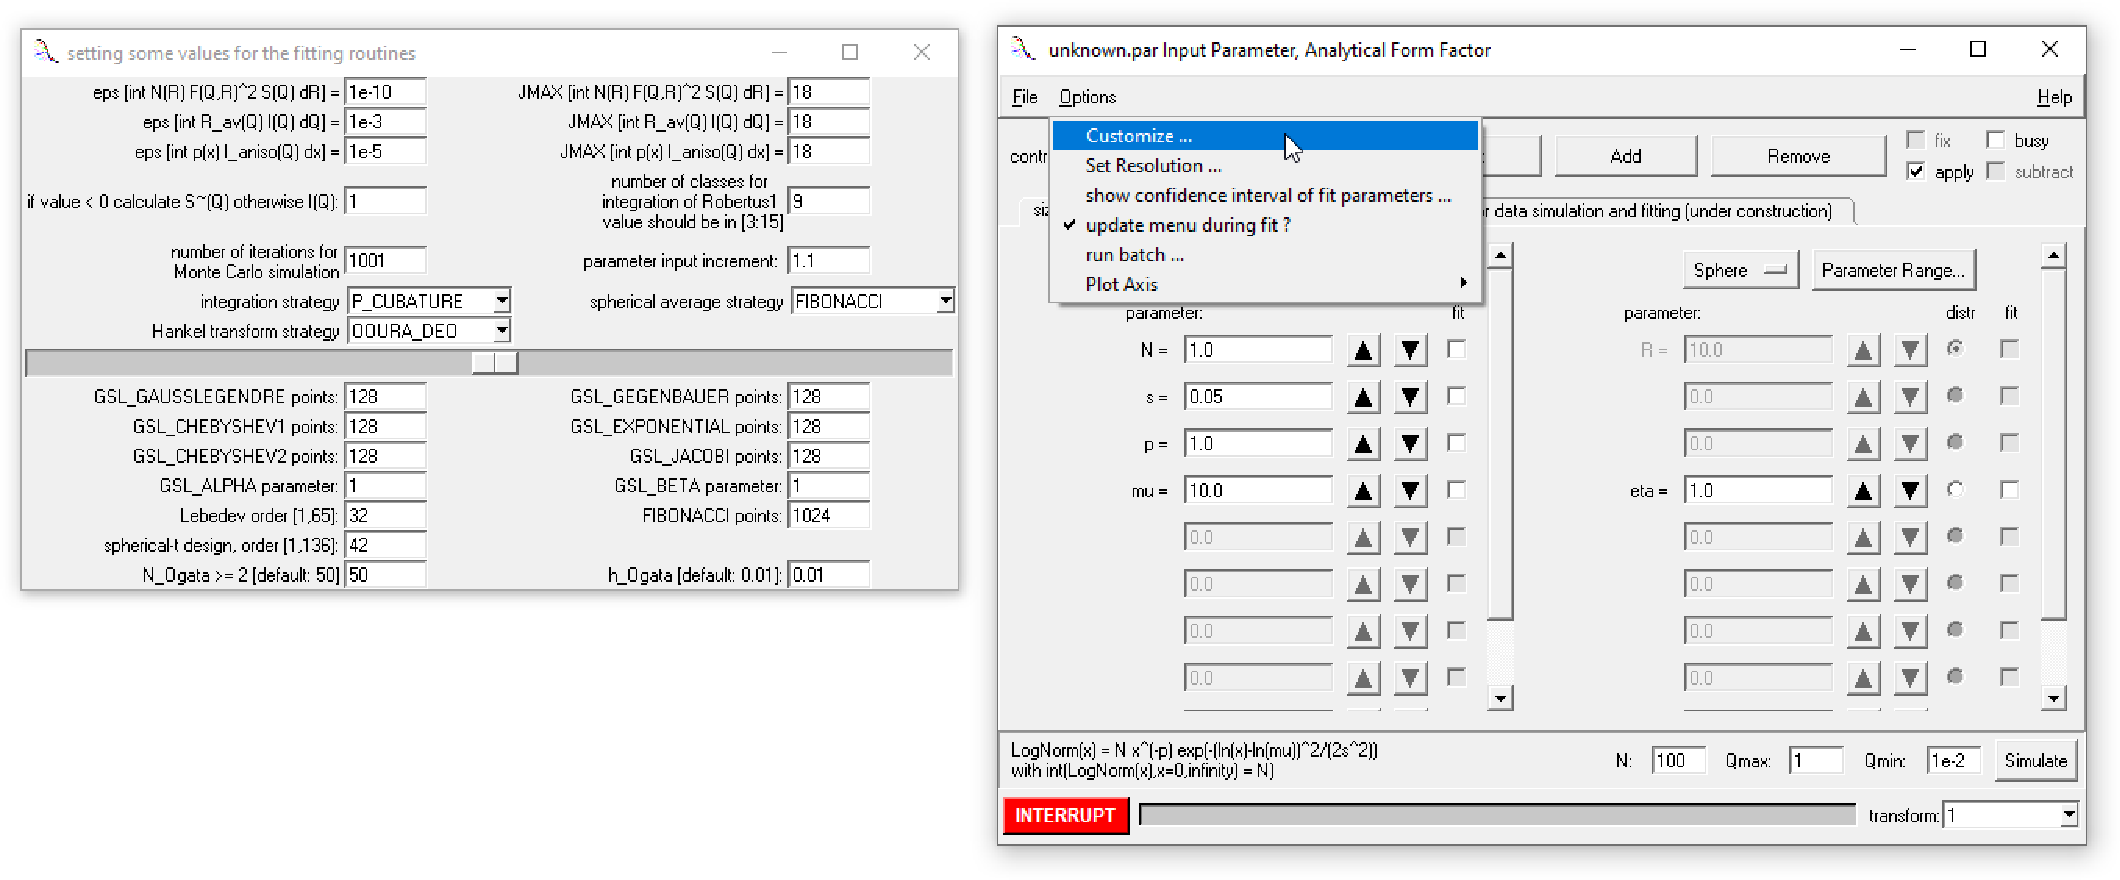
\includegraphics[width=0.95\textwidth]{../images/GUI/CustomizeWindow.pdf}
\end{center}
\caption{Menu for configuring internal integration routines in \SASfit}
\label{fig:CustomizeIntGUI}
\end{figure}

\subsection{Integration algorithms in SASfit for normal one- or multi-dimensional integration}  ~\\

Within \texttt{SASfit} a configurable one dimensional integration routine as well as a multidimensional one  with a common interface for the different algorithms is supplied. Depending on the mathematical behaviour of the integrant it has turned out that the different algorithms might differ a lot in terms of efficiency. For multidimensional quadrature algorithm so far the same strategy is used for all dimensions. The routines \texttt{sasfit\_integrate()}  and \texttt{sasfit\_cubature()} have the same configuration options. For multidimensional integrations either by itself specialized multidimensional algorithms or nested calls of one-dimensional integration routines are used. \\

\noindent Possible options for them are:\\
\begin{description}[font=\sffamily\bfseries, leftmargin=2.5cm,style=nextline,
                  nosep]
   \item[\texttt{OOURA\_DE}] double-exponential quadrature algorithm from \cite{Mori1990,Mori2001}
   \item[\texttt{OOURA\_CC}] Clenshaw-Curtis-quadrature using Chebyshev series expansion (\url{https://www.kurims.kyoto-u.ac.jp/~ooura/intcc.html})
   \item[\texttt{TANHSINH\_1}] TanhSinh quadrature \cite{Engelen2021,Engelen}
   \item[\texttt{TANHSINH\_2}] TanhSinh quadrature \cite{Engelen2021,Engelena}
   \item[\texttt{GSL\_QUAD}] quad integration routine from gsl \cite{Galassi2021}
   \item[\texttt{GSL\_QAG}] QAQ integration routine from gsl \cite{Galassi2021}
   \item[\texttt{GSL\_QNQ}] QNQ integration routine from gsl \cite{Galassi2021}
   \item[\texttt{H\_CUBATURE}] multidimensional integration routine \texttt{hcubature} from \cite{Johnson2017}
   \item[\texttt{P\_CUBATURE}] multidimensional integration routine \texttt{pcubature} from \cite{Johnson2017}
   \item[\texttt{GSL\_LEGENDRE}] Gauss-Legendre quadrature using gsl library  \cite{Galassi2021}
   \item[\texttt{MC\_MISER}] Monte-Carlo integration algorithm Miser using gsl library  \cite{Galassi2021}
   \item[\texttt{MC\_VEGAS}]  Monte-Carlo integration algorithm Vegas using gsl library  \cite{Galassi2021}
   \item[\texttt{MC\_PLAIN}]  plain Monte-Carlo integration algorithm using gsl library  \cite{Galassi2021}
   \item[\texttt{QMC\_HOLTON}] quasi Monte Carlo integration \cite{Zaslavsky2023} using the \texttt{gsl\_qrng\_halton} quasi random number generator from gsl \cite{Galassi2021}.
   \item[\texttt{QMC\_REVERSEHALTON}] quasi Monte Carlo integration \cite{Zaslavsky2023} using the \texttt{gsl\_qrng\_reversehalton} quasi random number generator from gsl \cite{Galassi2021}.
   \item[\texttt{QMC\_SOBOL}] quasi Monte Carlo integration \cite{Zaslavsky2023} using the \texttt{gsl\_qrng\_sobol} quasi random number generator from gsl \cite{Galassi2021}.
   \item[\texttt{QMC\_NIEDERREITER\_2}] quasi Monte Carlo integration \cite{Zaslavsky2023} using the reverse \texttt{gsl\_qrng\_niederreiter\_2} quasi random number generator from gsl \cite{Galassi2021}.
   \item[\texttt{RQMC\_SOBOL\_RDS}] randomized quasi Monte Carlo integration using the quasi random Sobol sequence with additional random digit scrambling \cite{Burley2020Scrambling}
   \item[\texttt{RQMC\_SOBOL\_OWEN}] randomized quasi Monte Carlo integration using the quasi random using Owen-scrambled Sobol sequence \cite{Burley2020Scrambling,Owen1995}
   \item[\texttt{RQMC\_FAURE05}] randomized quasi Monte Carlo integration using Owen-scrambled Faure (0,5) sequence \cite{Burley2020Scrambling,Owen1995}.
   \item[\texttt{RQMC\_LAINE\_KARRAS}] randomized quasi Monte Carlo integration using Laine-Karras hash method mentioned in \cite{Burley2020Scrambling} and given as C source code in its supplement information.
   \item[\texttt{SG\_SMOLYAK}] A sparse grid is used, based on a "delayed" Clenshaw Curtis quadrature rule, using the Smolyak method \cite{Petras2003,Burkardt2019}.
   \item[\texttt{SG\_CC\_SMOLYAK}] A sparse grid is used, based on a Clenshaw Curtis quadrature rule, using the Smolyak method \cite{Petras2003,Burkardt2019}.
   \item[\texttt{SG\_SMOLYAK\_CLENSHAW\_CURTIS}] The quadrature rule is associated with a sparse grid derived from a Smolyak construction using a closed 1D quadrature rule \cite{Nobile2008,Burkardt2019}.
   \item[\texttt{SG\_CLENSHAW\_CURTIS\_LINEAR}] sparse grid based on Clenshaw Curtis quadrature rule \cite{Heiss2008,Heiss2025,Burkardt2019a}
   \item[\texttt{SG\_CLENSHAW\_CURTIS\_SLOW}] sparse grid based on "slow growth" Clenshaw Curtis quadrature rule \cite{Heiss2008,Heiss2025,Burkardt2019a}
   \item[\texttt{SG\_CLENSHAW\_CURTIS\_EXP}] sparse grid based on Clenshaw-Curtis Exponential quadrature rule \cite{Heiss2008,Heiss2025,Burkardt2019a}
   \item[\texttt{SG\_GAUSS\_LEGENDRE}] sparse grids based on Gauss-Legendre rules\cite{Heiss2008,Heiss2025,Burkardt2019a}
   \item[\texttt{SG\_KONROD\_PATTERSON}]sparse grids based on \ Gauss-Patterson rules\cite{Heiss2008,Heiss2025,Burkardt2019a}
   \item[\texttt{SG\_FROLOV}]  sparse grids using optimized Frolov lattices \cite{Kacwin2020,InstitutfuerNumerischeSimulation2025}
\end{description}


\section{orientation average} ~\\

Orientational averaging is a two dimensional integration over a unit sphere (\texttt{sasfit\_orient\_avg()}). In \texttt{SASfit} a specialized function for this is supplied. As the problem in principle can be handles with \texttt{sasfit\_cubature} it include all strategies from that function plus a few specialized one especially efficient for quadrature over a the surface of unit sphere. These are
\begin{description}
\item[\texttt{Lebedev}] Lebedev quadrature \cite{WikiLebedevQuad2024,Lebedev1975,Lebedev1976,Lebedev1977,Lebedev2003} is an approximation to the surface integral of a function over a three-dimensional sphere. The number and location of the grid points together with a corresponding set of integration weights are determined by enforcing the exact integration of polynomials (or equivalently, spherical harmonics) up to a given order.
\item[\texttt{FIBONACCI}]  Almost equally spaced points can be easily generated by a Fibonacci on different surfaces, like square, disk, cylinder surface, spherical surface \cite{Marques_2013,Swinbank2006}.
\item[\texttt{spherical\_t\_design}] The spherical t-design \cite{WikipediaSphericalDesign2024,Graef2011,Hardin1996} has been used to generate equally spaced points on a spherical surface leading to a quadrature formula with equal weights.
\end{description}

\subsection{Hankel transform} ~\\

The Hankel transform calculated by \texttt{sasfit\_hankel()} is defined by
\begin{align}\label{eq:HT}
F(q) &= \mathcal{H}_n\left[f(q)\right](r)  = \int_0^\infty \mathrm{J}_n(qr) f(r) r \mathrm{d}r
\end{align}
This means an upper unbounded integral over the oscillating Bessel function $\mathrm{J}_n()$ has to be solved numerically.
Thos strategies already available for functions with an strictly periodic $\cos()$ or $\sin()$ term (Fourier type) can not be directly been used as only for large arguments of the bessel function in behaves as $\mathrm{J}_n(x)\approx \sqrt{\frac{2}{\pi x}}\cos\left(x-\frac{\pi}{2}n-\frac{\pi}{4}\right)$.
\begin{description}
\item[\texttt{QWE}] Quadrature With Extrapolation computes an
infinite integral using the partial sum of quadrature terms
accelerated by sequence extrapolation using the Shanks transformation
implemented with Wynn's epsilon algorithm \cite{Key2012}.
\item[\texttt{CHAVE}]  This algorithm performs the integration of the product of the kernel and Bessel functions between the asymptotic zero crossings of the latter and sums the series of partial integrations using a continued fraction expansion, equivalent to an analytic continuation of the series \cite{Chave1983}.
\item[\texttt{OOURA\_DEO}] As for large arguments $x$ the Bessel function asymptotically behaves as
$\mathrm{J}_n\approx \sqrt{\frac{2}{\pi x}}\cos\left(x-\frac{\pi}{2}n-\frac{\pi}{4}\right)$ the double exponential formula of \cite{Ooura_1991} for oscillatory functions over the half infinite interval is used directly.
\item[\texttt{GSL\_QAWF}] This options tries to make use of the adaptive integration of Fourier integrals available in the gsl library (\texttt{gsl\_integration\_qawf()}). This function attempts to compute a Fourier integral of the function $g$ over the semi-infinite interval $[a,+\infty)$ as
$I = \int_a^{+\infty} \mathrm{d}x g(x)
\left\{
\begin{array}{c}
\sin{(\omega x)} \\
\cos{(\omega x)}
\end{array}
\right\}$
By defining $g(r)= f(r) \frac{\mathrm{J}_n(qr)}{\cos\left(qr-\frac{\pi}{2}n-\frac{\pi}{4}\right)}$ we convert the Hankel transform in \ref{eq:HT} into a $\cos$-Fourier type transform after an additional substitutions of $r'=r-\frac{\pi}{2}\frac{n}{q}-\frac{1}{q}\frac{\pi}{4}$.
\end{description}
Next to the quadrature algorithms above also fast digital filters for Hankel transform have been developed. A few of these have been supplied in SASfit for testing \cite{Anderson1989,Guptasarma1997,Ogata2005,Kong2007,Key2012,Kang2021}: \\
\texttt{OGATA\_2005}, \texttt{FBT0}, \texttt{FBT1}, \texttt{FBT2}, \texttt{GUPTASARMA\_97}, \texttt{GUPTASARMA\_97\_FAST}, \texttt{KEY\_51}, \texttt{KEY\_101}, \texttt{KEY\_201}, \texttt{ANDERSON\_801}



\clearpage
\section{Fitting strategies}
